\documentclass[11pt]{beamer}
\usetheme{CambridgeUS}
\usepackage[utf8]{inputenc}
\usepackage{amsmath}
\usepackage{amsfonts}
\usepackage{amssymb}
\usepackage{graphicx}
\usepackage{pgfpages}
\usepackage{framed}
\usepackage{xcolor}
\usepackage[most]{tcolorbox}
\usepackage{soul}
\usepackage{empheq}
\usepackage{booktabs}
\usepackage{listings}

% The replacement character � (often displayed as a black rhombus with a white
% question mark) is a symbol found in the Unicode standard at code point U
% +FFFD in the Specials table. It is used to indicate problems when a system 
% is unable to render a stream of data to a correct symbol.[4] It is usually 
% seen when the data is invalid and does not match any character. For this 
% reason we map explicitly this character to a blanck space.
\DeclareUnicodeCharacter{FFFD}{ }

\newcommand*{\itemimg}[1]{%
  \raisebox{-.3\baselineskip}{%
    \includegraphics[
      height=\baselineskip,
      width=\baselineskip,
      keepaspectratio,
    ]{#1}%
  }%
}

\newtcbox{\mymath}[1][]{%
    nobeforeafter, math upper, tcbox raise base,
    enhanced, colframe=blue!30!black,
    colback=blue!10, boxrule=1pt,
    #1}

\newcommand{\highlight}[1]{%
  \colorbox{yellow!50}{$\displaystyle#1$}}

\author{Giovanni Della Lunga\\{\footnotesize giovanni.dellalunga@unibo.it}}
%\title{1.1 - Introduction to Machine Learning}
%\title{1.2 - Data Gathering with Pandas}
\title{1.4 - Data Pre-Processing}
%\title{4.1 - Linear and Logistic Regression}
%\title{4.2 - Decision Trees}
%\title{6 - Text Vectorization}
%\title{7 - Classification for Text Analysis}
%\title{8 - Clustering for Text Similarity}
%\title{9 - Information Extraction}
\subtitle{} % (optional)
\setbeamercovered{transparent} 
\institute{Introduction to Machine Learning for Finance} 
\date{Bologna - February-March, 2025} 

\begin{document}

%\begin{frame}
%\includegraphics[width=\linewidth]{img/halloween-seminar-logo.PNG}
%\end{frame}

\begin{frame}
\titlepage
\end{frame}

\AtBeginSection[]
{
  %\begin{frame}<beamer>
  %\footnotesize	
  %\frametitle{Outline}
  %\begin{multicols}{2}
  %\tableofcontents[currentsection]
  %\end{multicols}	  
  %\normalsize
  %\end{frame}
  \begin{frame}
  \vfill
  \centering
  \begin{beamercolorbox}[sep=8pt,center,shadow=true,rounded=true]{title}  	\usebeamerfont{title}\insertsectionhead\par%
  \end{beamercolorbox}
  \vfill
  \end{frame}
}
\AtBeginSubsection{\frame{\subsectionpage}}
%
%---------------------------------------------------------------------------------------------------
%
\section{Data Pre-Processing}
%
%---------------------------------------------------------------------------------------------------
%
\begin{frame}
\begin{center}

\includegraphics[scale=.75]{../05-pictures/lesson-1-4_pic_9.png} 
\end{center}
\end{frame}
%
%..................................................................
%
\begin{frame}{Introduction}{Data Pre-Processing}
\begin{itemize}
\item Before applying any machine learning model, it is essential to establish a rigorous understanding of \textbf{data pre-processing}.  
\item Poorly prepared data can lead to misleading conclusions, rendering even the most sophisticated algorithms ineffective.

\item Data pre-processing introduces several key concepts that are \textbf{transversal to all of machine learning}; among these, \textbf{handling missing values}, \textbf{feature scaling}, \textbf{encoding categorical variables}, and \textbf{detecting outliers} are crucial. 

\item These techniques ensure that the input data is structured, consistent, and suitable for training robust models. 

\item Without proper data preparation, models may struggle with convergence, exhibit bias, or fail to generalize to new data.

\end{itemize}
\end{frame}
%
%..................................................................
%
\begin{frame}{Introduction}{Data Pre-Processing}
In this lesson, we will cover the essential components of data pre-processing, including:

\begin{itemize}
\item Handling missing data: imputation and removal strategies
\item Feature scaling: normalization and standardization
\item Encoding categorical variables
\item Detecting and handling outliers
\item Feature Selection and Dimensionality Reduction
\end{itemize}
\end{frame}
%
%..................................................................
%
\begin{frame}{Data Pre-Processing}
	\begin{itemize}
		\item Raw data rarely comes in the form and shape that is necessary for the optimal performance of a learning algorithm. 
		\item On the other hand, the success of a machine learning algorithm highly depends on the quality of the data fed into the model. 
		\item Real-world data is often dirty containing outliers, missing values, wrong data types, irrelevant features, or non-standardized data. 
		\item The presence of any of these will prevent the machine learning model to properly learn. 
		\item For this reason, transforming raw data into a useful format is an essential stage in the machine learning process. 
	\end{itemize}
\end{frame}
%
%..................................................................
%
\begin{frame}{Data Cleaning}
	\begin{itemize}
		\item Dealing with inconsistent recording
		\item Removing unwanted observations
		\item Removing duplicates
		\item Investigating outliers
		\item Dealing with missing items
	\end{itemize}
\end{frame}
%
%---------------------------------------------------------------------------------------------------
%
\subsection{Missing Data \\ \scalebox{0.8}{}}
%
%---------------------------------------------------------------------------------------------------
%
\begin{frame}{Dealing with Missing Data}
	\begin{itemize}
		\item The real-world data often has a lot of missing values. 
		\item The cause of missing values can be data corruption or failure to record data. 
		\item The handling of missing data is very important during the preprocessing of the dataset as many machine learning algorithms do not support missing values.
	\end{itemize}
\end{frame}
%
%..................................................................
%
\begin{frame}{Dealing with Missing Data}
\textbf{Delete Rows/Columns with Missing Values} 
\begin{itemize}
\item One of the easiest ways to deal with missing data is simply to remove the
corresponding features (columns) or training examples (rows) from the dataset
entirely; 
\item Missing values can be handled by deleting the rows or columns having null values. If columns have more than half of the rows as null then the entire column can be dropped.
\ The rows which are having one or more columns values as null can also be dropped.
\item  Remember that, in pandas, rows with missing values can easily be dropped via the \textbf{dropna} method.
\end{itemize}
\end{frame}
%
%..................................................................
%
\begin{frame}{Dealing with Missing Data}
\textbf{Delete Rows/Columns with Missing Values} \\
\vspace{0.5cm}
\textbf{Pros}:
\begin{itemize}
\item A model trained with the removal of all missing values creates a robust model.
\end{itemize}
\textbf{Cons}:
\begin{itemize}
\item Loss of a lot of information.
\item Works poorly if the percentage of missing values is excessive in comparison to the complete dataset.
\end{itemize}
\end{frame}
%
%..................................................................
%
\begin{frame}{Dealing with Missing Data}
\textbf{Imputing missing values with Mean/Median}:
\begin{itemize}
\item Columns in the dataset which have numeric continuous values can be replaced with the mean, median, or mode of remaining values in the column. 
\item This method can prevent the loss of data compared to the earlier method. 
\end{itemize}
\end{frame}
%
%..................................................................
%
\begin{frame}{Dealing with Missing Data}
\textbf{Imputing missing values with Mean/Median}\\
\vspace{0.5cm}
\textbf{Pros}:
\begin{itemize}
\item Prevent data loss which results in deletion of rows or columns
\item Works well with a small dataset and is easy to implement.
\end{itemize}
\textbf{Cons}:
\begin{itemize}
\item Works only with numerical continuous variables.
\item Can cause data leakage
\item Do not factor the covariance between features.
\end{itemize}
\end{frame}
%
%---------------------------------------------------------------------------------------------------
%
\subsection{Categorical Data \\ \scalebox{0.8}{}}
%
%---------------------------------------------------------------------------------------------------
%
\begin{frame}{What is Categorical Data?}
\textbf{Definitions}
\vspace{0.5cm}
	\begin{itemize}
		\item Categorical data refers to data that consists of discrete labels or categories rather than numerical values. 
		\item These categories represent different groups or classifications, such as colors (red, blue, green), gender (male, female, non-binary), or product types (electronics, clothing, furniture). 
		\item There are two types of categorical variables:\\ \vspace{0.5cm}
		- \textbf{I. Ordinal Variables}  \\
\vspace{0.5cm}
		- \textbf{II. Nominal Variables}
	\end{itemize}
\end{frame}
%
%..................................................................
%
\begin{frame}{Categorical Data: Ordinal Variables}
\textbf{Ordinal Variables}
	\begin{itemize}
		\item These variables maintain a natural order in their class of values. 
		\item If we consider the level of education then we can easily sort them according to their education tag in the order of \textit{High School} < \textit{ Under-Graduate} < \textit{ post-Graduate} < \textit{ PhD}. 
		\item The review rating system can also be considered as an ordinal data type where 5 stars is definitely better than 1 star.
	\end{itemize}
\begin{center}
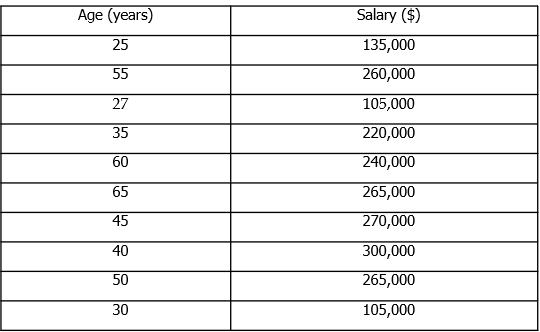
\includegraphics[scale=.4]{../05-pictures/lesson-2-1_pic_0.png} 
\end{center}	
\end{frame}
%
%..................................................................
%
\begin{frame}{Categorical Data in Credit Scoring}
    
    \begin{table}[]
        \centering
        \renewcommand{\arraystretch}{1.5} % Increase row height
        \begin{tabular}{|c|c|c|}
            \hline
            \rule{0pt}{15pt} % Extra space before column headers
            \textbf{Applicant ID} & \textbf{Employment Type} & \textbf{Credit Rating} \\
            \hline
            001 & Salaried & AAA \\
            002 & Self-Employed & BBB \\
            003 & Unemployed & C \\
            004 & Salaried & A \\
            \hline
        \end{tabular}
        \vspace{0.5cm}
        \caption{Example of Categorical Data in Credit Scoring}
    \end{table}
    
\end{frame}
%
%..................................................................
%
\begin{frame}{Categorical Data: Nominal Variables}
\textbf{Nominal Variables}
	\begin{itemize}
		\item These variables do not maintain any natural/logical order. 
		\item The color of a car can be considered as Nominal Variable as we cannot compare the color with each other. 
		\item It is impossible to state that \textbf{\textit{Red}} is better than \textbf{\textit{Blu}} (subjective!). 
		\item Similarly, Gender is a type of Nominal Variable as again we cannot differentiate between Male, Female, and Others.
	\end{itemize}
\begin{center}
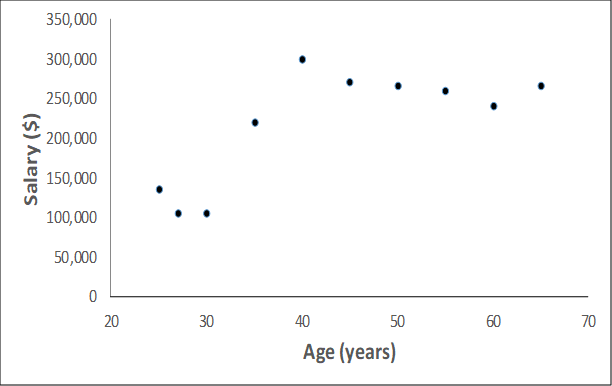
\includegraphics[scale=.5]{../05-pictures/lesson-2-1_pic_1.png} 
\end{center}	
\end{frame}
%
%..................................................................
%
\begin{frame}{Categorical Data: Encoding}
	\begin{itemize}
		\item Most of the Machine learning algorithms are designed to work with numeric data. 
		\item Hence, we need to convert Categorical (text) data into numerical data for model building. 
		\item There are multiple encoding techniques to convert categorical data into numerical data. Let us look at some of them.
	\end{itemize}
\end{frame}
%
%..................................................................
%
\begin{frame}{Categorical Data: Ordinal Encoding}
	\begin{itemize}
		\item \textbf{Ordinal Encoding} primarily encodes ordinal categories into ordered numerical values. 
		\item Ordinal encoding maps each unique category value to a specific numerical value based on its order or rank. 
		\item Consider for example the credit risk table. 
		\item Here, we can define the ordering of the customer based on their creditworthiness using the OrdinalEncoder methods of  
		\item \textit{OrdinalEncoder(categories=[['AAA', 'AA', 'A', 'B+', ...]])}
	\end{itemize}
\end{frame}
%
%..................................................................
%
\begin{frame}[fragile]{Ordinal Encoding - Python Code}
    \textbf{Python Implementation:}
\footnotesize{
    \begin{verbatim}
from sklearn.preprocessing import OrdinalEncoder

ratings = [["AAA", "AA", "A", "BBB", "BB", "B", "CCC", "CC", "C", "D"]]

le = OrdinalEncoder(categories=ratings)
df["rating_encoded"] = le.fit_transform(df[["rating"]])
df.head()    
\end{verbatim}
    }
\end{frame}
%
%..................................................................
%
\begin{frame}{Categorical Data: Label Encoding}
	\begin{itemize}
		\item The label encoder will convert each category into a unique numerical value. 
		\item If implemented with Sklearn, then this encoder should be used to encode output values, i.e. y, and not the input X. 
		\item It is similar to the ordinal encoder except, here the numeric values are assigned automatically without following any sort of natural order. 
		\item Generally, the alphabetical order of the categorical values is used to determine which numerical value comes first. 
	\end{itemize}
\end{frame}
%
%..................................................................
%
\begin{frame}{Categorical Data: Label Encoding}
	\begin{itemize}
		\item Consider for example a target variable 'Job Status' that has four different categories. 
		\item After applying label encoding to this column the four different categories are mapped into integers 0: Full Time, 1: Intern, 2: Part-Time, and 3:Unemployed. 
		\item With this, it can be interpreted that Unemployed have a higher priority than Part-Time, Full Time, and Intern while training the model, whereas, \textbf{there is no such priority or relation between these statuses}. 
		\item We cannot define the order of labels with the label encoding technique.
	\end{itemize}
\end{frame}
%
%..................................................................
%
\begin{frame}{Categorical Data: Label Encoding}
	\begin{center}
	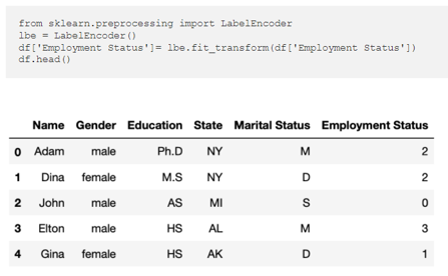
\includegraphics[scale=1]{../05-pictures/lesson-2-1_pic_3.png}
	\end{center}
\end{frame}
%
%..................................................................
%
\begin{frame}{Comparison Between Ordinal and Label Encoding}
    \begin{itemize}
        \item Both \textbf{Ordinal Encoding} and \textbf{Label Encoding} convert categorical data into numbers.
        \item However, they serve \textbf{different purposes} and should not be used interchangeably.
    \end{itemize}
\end{frame}
%
%..................................................................
%
\begin{frame}{Ordinal Encoding}{Comparison Between Ordinal and Label Encoding}
    \textbf{Concept:}
    \begin{itemize}
        \item Assigns an integer to each category \textbf{based on a predefined order}.
        \item \textbf{Preserves order} in the data.
    \end{itemize}
    \vspace{0.3cm}
    \textbf{Example: Credit Ratings}
    \begin{table}[]
        \centering
        \begin{tabular}{ll}
            \toprule
            \textbf{Rating} & \textbf{Ordinal Encoding} \\
            \midrule
            CCC & 0 \\
            B   & 1 \\
            BB  & 2 \\
            BBB & 3 \\
            A   & 4 \\
            AA  & 5 \\
            AAA & 6 \\
            \bottomrule
        \end{tabular}
    \end{table}
\end{frame}
%
%..................................................................
%
\begin{frame}{Label Encoding}{Comparison Between Ordinal and Label Encoding}
    \textbf{Concept:}
    \begin{itemize}
        \item Assigns a unique integer to each category, but \textbf{without any ordering}.
        \item Numbers \textbf{do not represent a ranking}.
    \end{itemize}
    \vspace{0.3cm}
    \textbf{Example: Car Brands}
    \begin{table}[]
        \centering
        \begin{tabular}{ll}
            \toprule
            \textbf{Car Brand} & \textbf{Label Encoding} \\
            \midrule
            Toyota & 0 \\
            Ford   & 1 \\
            BMW    & 2 \\
            Tesla  & 3 \\
            \bottomrule
        \end{tabular}
    \end{table}
\end{frame}
%
%..................................................................
%
\begin{frame}[fragile]{Label Encoding - Python Code}{Comparison Between Ordinal and Label Encoding}
    \textbf{Python Implementation:}
    \footnotesize{
    \begin{verbatim}
from sklearn.preprocessing import LabelEncoder

data = pd.DataFrame({'car_brand': ['Toyota', 'Ford', 
                     'BMW', 'Tesla', 'Ford']})
encoder = LabelEncoder()
data['brand_encoded'] = encoder.fit_transform(data['car_brand'])
print(data)
    \end{verbatim}
}
\end{frame}
%
%..................................................................
%
\begin{frame}{Key Differences}{Comparison Between Ordinal and Label Encoding}
    \textbf{Comparison Table}
%\footnotesize{
    \begin{table}[]
        \centering
        \begin{tabular}{lll}
            \toprule
            \textbf{Feature} & \textbf{Ordinal Encoding} & \textbf{Label Encoding} \\
            \midrule
            Preserves Order?  & Yes & No  \\
            Use Case         & Ordered Categories & Unordered \\
            Assigns Numbers?  & Yes & Yes \\
            Represents Ranking? & Yes & No \\
            Risk of Misinterpretation? & If order is wrong & If used on ordered data \\
            Scikit-Learn Class & OrdinalEncoder & LabelEncoder \\
            \bottomrule
        \end{tabular}
    \end{table}
%    }
\end{frame}
%
%..................................................................
%
\begin{frame}{Conclusions}{Comparison Between Ordinal and Label Encoding}
    \begin{itemize}
        \item Use \textbf{Ordinal Encoding} only when categories have a meaningful order.
        \item Use \textbf{Label Encoding} for nominal data where order does not matter.
        \item Consider alternative encoding methods (e.g., \textbf{One-Hot Encoding}) for categorical variables with many unique values.
    \end{itemize}
\end{frame}
%
%..................................................................
%
\begin{frame}{Categorical Data: One Hot Encoding}

\textbf{What is One Hot Encoding?}

	\begin{itemize}
		\item if there is no ordinal relationship between the categorical variables then ordinal encoding might mislead the model. 
		\item This is because the ordinal encoder will try to force an ordinal relationship on the variables to assume a natural ordering, thus resulting in poor performance.
		\item In this case, One Hot encoder should be used to treat our categorical variables. 
		\item It will create dummy variables by converting N categories into N features/columns. 
	\end{itemize}
\end{frame}
%
%..................................................................
%
\begin{frame}{Original Binary Variable}{Categorical Data: One Hot Encoding}
\textbf{A binary variable example that illustrates one-hot encoding is "Has Mortgage"}, where applicants either have a mortgage (\texttt{Yes}) or do not (\texttt{No}).
    \begin{table}[]
        \centering
        \renewcommand{\arraystretch}{1.5} % Increase row height
        \begin{tabular}{|c|c|}
            \hline
            \rule{0pt}{15pt} % Extra space before column headers
            \textbf{Applicant ID} & \textbf{Has Mortgage} \\
            \hline
            001 & Yes \\
            002 & No \\
            003 & Yes \\
            004 & No \\
            \hline
        \end{tabular}
        \caption{Original Binary Variable}
    \end{table}
\end{frame}
%
%..................................................................
%
\begin{frame}{After One-Hot Encoding}{Categorical Data: One Hot Encoding}
\textbf{A binary variable example that illustrates one-hot encoding is "Has Mortgage"}, where applicants either have a mortgage (\texttt{Yes}) or do not (\texttt{No}).
    \begin{table}[]
        \centering
        \renewcommand{\arraystretch}{1.5} % Increase row height
        \begin{tabular}{|c|c|c|}
            \hline
            \rule{0pt}{15pt} % Extra space before column headers
            \textbf{Applicant ID} & \textbf{Has Mortgage (Yes)} & \textbf{Has Mortgage (No)} \\
            \hline
            001 & 1 & 0 \\
            002 & 0 & 1 \\
            003 & 1 & 0 \\
            004 & 0 & 1 \\
            \hline
        \end{tabular}
        \caption{One-Hot Encoded Binary Variable}
    \end{table}
\end{frame}
%
%..................................................................
%
\begin{frame}{After One-Hot Encoding}{Categorical Data: One Hot Encoding}
We can one-hot encode categorical variables in two ways: by using \textbf{get\_dummies} in pandas and by using \textbf{OneHotEncoder} from sklearn.
    \begin{table}[]
        \centering
        \renewcommand{\arraystretch}{1.5} % Increase row height
        \begin{tabular}{|c|c|c|}
            \hline
            \rule{0pt}{15pt} % Extra space before column headers
            \textbf{Applicant ID} & \textbf{Has Mortgage (Yes)} & \textbf{Has Mortgage (No)} \\
            \hline
            001 & 1 & 0 \\
            002 & 0 & 1 \\
            003 & 1 & 0 \\
            004 & 0 & 1 \\
            \hline
        \end{tabular}
        \caption{One-Hot Encoded Binary Variable}
    \end{table}
\end{frame}
%
%---------------------------------------------------------------------------------------------------
%
\subsection{Feature Scaling (Normalization) \\ \scalebox{0.8}{}}
%
%---------------------------------------------------------------------------------------------------
%
\begin{frame}{Feature Scaling}
	\begin{itemize}
		\item Before using many ML algorithms (including those for unsupervised learning), it is important to scale feature values so that they are comparable.
		\item  Z-score scaling involves calculating the mean ($\mu$) and SD ($\sigma$) from the values of each feature from the training set. Scaled feature values for all data sets are then created by subtracting the mean and dividing by the SD. 
\item The scaled feature values have a mean of zero and SD of one.
		\begin{equation}
		\text{scaled feature value} = \frac{V-\mu}{\sigma}
		\end{equation}
	\end{itemize}
\end{frame}
%
%..................................................................
%
\begin{frame}{Feature Scaling}
	\begin{itemize}
		\item Min-max scaling involves calculating the maximum and minimum value of each feature from the training set. 
		\item Scaled feature values for all data sets are then created by subtracting the minimum and dividing by the difference between the maximum and minimum. 
		\item The scaled feature values lie between zero and one:
		
				\begin{equation}
		\text{scaled feature value} = \frac{V-V_{min}}{V_{max}-V_{min}}
		\end{equation}
	\end{itemize}
\end{frame}
%=====================================================================
\end{document}
%=====================================================================

%..................................................................
\begin{frame}{Standardization and Gradient Descent}
	\begin{center}
	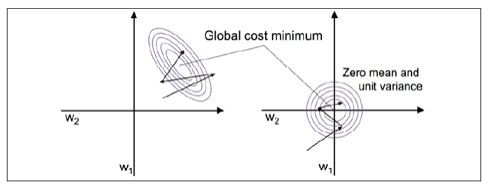
\includegraphics[scale=1]{../05-pictures/lesson-2-1_pic_4.png}
	\end{center}
\end{frame}
%
%..................................................................
%
\begin{frame}{Introduction}{Data Pre-Processing}
\begin{itemize}
\item
\end{itemize}
\end{frame}
%
%..................................................................
%
\begin{frame}{Introduction}{Data Pre-Processing}
\begin{itemize}
\item
\end{itemize}
\end{frame}
